\problem{What is zero shifting by partial removal of a pole? Explain with a suitable example.}
The partial removal of a pole means the removal of some fraction of the total network, removing which would not destroy the positive, real nature of the function.\\
A lossless function in partial form is given as,
\begin{equation}
    Z(s)=Hs+\frac{K_o}{s}+\sum_{i=1}^{n}\frac{2K_is}{s^2+\omega_i^2}
    \label{eqn:partial-rep}
\end{equation}
\subsubsection*{Weakening pole at infinity}
The term $Hs$ in Equation~\ref{eqn:partial-rep} is contributed by pole at infinity. Since we are concerned with partial removal of this pole, we subtract a $K_p$ fraction of $Hs$ from $Z(s)$ as,
\begin{equation*}
    Z_1(s)=Z(s)-K_pHs \quad [K_p<1]
\end{equation*}
Since the zeros of $Z_1(s)$ are still located on the $j\omega$ axis, we substitute $s=j\omega$ to find them as,
\begin{equation*}
    X_1(\omega)=X(\omega)-K_pH\omega \quad
    [\because Z_1(j\omega)=jX_1(\omega)]
\end{equation*}
The zeros of $X_1(\omega)$ are the values of $\omega$ satisfying
\begin{equation*}
    X(\omega)=K_pH\omega
\end{equation*}
\begin{figure}[H]
    \centering
    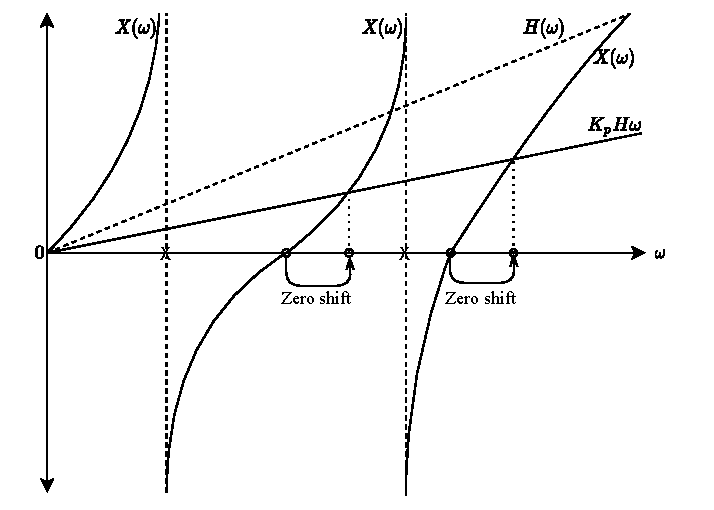
\includegraphics{../Figures/zero_shifting_by_weakening_pole_at_inf}
    \caption{Zero shifting by weakening pole at infinity}
    \label{fig:pole-inf}
\end{figure}

\subsubsection*{Weakening pole at origin}
The term $\ddfrac{K_o}{s}$ in Equation~\ref{eqn:partial-rep} is contributed by pole at origin. Since we are concerned with partial removal of this pole, we subtract a $K_p$ fraction of $\ddfrac{K_o}{s}$ from $Z(s)$ as,
\begin{equation*}
    Z_2(s)=Z(s)-K_p\frac{K_o}{s} \quad [K_p<1]
\end{equation*}
Similarly, the zeros of this function can be located by the intersection of $X(\omega)$ and $-K_p\left(\ddfrac{K_o}{\omega}\right)$ with $\omega$ as they must satisfy,
\begin{equation*}
    X(\omega)=-K_p\left(\frac{K_o}{\omega}\right)
\end{equation*}
\begin{figure}[H]
    \centering
    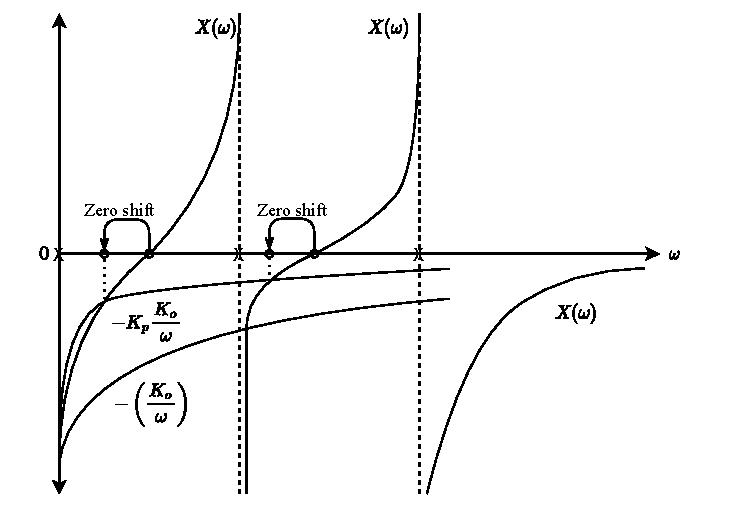
\includegraphics{../Figures/zero_shifting_by_weakening_pole_at_org}
    \caption{Zero shifting by weakening pole at origin}
    \label{fig:pole-org}
\end{figure}

\subsubsection*{Weakening pole at complex conjugate pair}
The term $\ddfrac{2K_is}{s^2+\omega_i^2}$ in Equation~\ref{eqn:partial-rep} is contributed by pole at a finite non-zero location. Since we are concerned with partial removal of this pole, we subtract a $K_p$ fraction of $\ddfrac{2K_is}{s^2+\omega_i^2}$ from $Z(s)$ as,
\begin{equation*}
    Z_3(s)=Z(s)-K_p\ddfrac{2K_is}{s^2+\omega_i^2} \quad [K_p<1]
\end{equation*}
Similarly, the zeros of this function can be located by the intersection of $X(\omega)$ and $-K_p\left(\ddfrac{2K_is}{\omega^2-\omega_i^2}\right)$ with $\omega$ as they must satisfy,
\begin{equation*}
    X(\omega)=-K_p\left(\ddfrac{2K_is}{\omega^2-\omega_i^2}\right)
\end{equation*}
\begin{figure}[H]
    \centering
    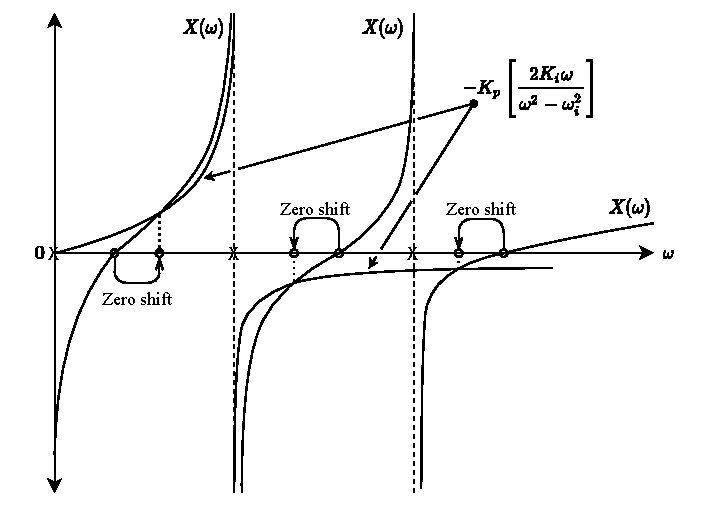
\includegraphics{../Figures/zero_shifting_by_weakening_pole_at_finite}
    \caption{Zero shifting by weakening pole at complex conjugate pair}
    \label{fig:pole-fin}
\end{figure}
To summarize,
\begin{enumerate}
    \item The partial removal of a pole shifts the zero towards that pole.
    \item The zero shift amount depends on the value of $K_p$ and proximity of zero to that pole.
    \item The partial removal of pole at origin doesn't affect zero at infinity and vice versa.
    \item A zero can never be shifted beyond an adjacent pole, rather it can be shifted a fraction of that distance.
\end{enumerate}